\documentclass[a4paper]{article}

\usepackage[english]{babel}
\usepackage[utf8]{inputenc}
\usepackage{amsmath}
\usepackage{graphicx}
\usepackage[colorinlistoftodos]{todonotes}
\usepackage[export]{adjustbox}[2011/08/13]
\usepackage{float}
\usepackage{bm}

\title{Behaviour Dynamics in Social Networks - Assignment 5}

\author{Maria Hotoiu, Federico Tavella}

\date{\today}

\begin{document}
\maketitle

\begin{abstract}
In this assignment the idea is to teach you how to work with social analysis software and data mining with social media data.
\end{abstract}

\section{The dining-table partners Network}

\subsection{Question 1}

The average degree value is 2.0. It is a logical value because every girl has to choose two options. The highest in-degree value is 6 and two nodes have this value. In this context, the in-degree indicates by how many girls that person was choosen as a dining partner. The most isolated people are the ones that have in-degree equal to zero (i.e. Alice, Ella, Irene, Laura and Ruth). The most important people in the network are the ones with the highest in-degree value, like Eva and Marion. We choose the people with the highest in-degree value because we think that they are the most influential and thus they can ispire the highest number of people.

\subsection{Question 2}

Using a representation that helps us to highlight the in-degree of each node can help us to identify the most isolated (i.e. the smallest ones) and the most popular nodes (i.e. the biggest ones).

Some different metrics to define the position of a person in the network could be the degree and also the out-degree because they are indicators of how much a person is connected to the rest of the network.

\subsection{Question 3}

There are 11 strongly connected components. There is only one weakly connected components because once the edges are undirected the whole graph become connected. Looking at the color of the nodes, we can identify which are the most isolated nodes: they are the only ones that are not connected to a node of the same color as their own. They are the same as the ones identified previously. We can also identify the nodes that can play a very influential role in the network by looking for the most spread color: this indicates the size of the strongly connected components, thus the number of nodes we can influence starting from one of them.

\begin{figure}[!htpb]
\centering
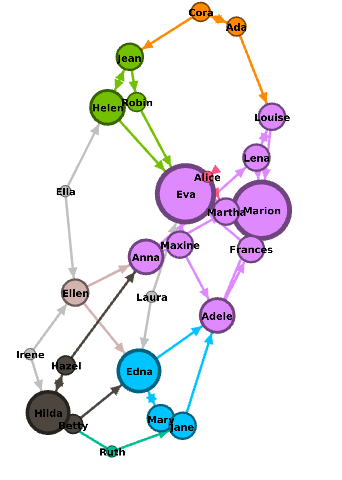
\includegraphics[width=0.55\textwidth]{res/img/graph}
\caption{Strongly connected components}
\label{fig:graph}
\end{figure}

\subsection{Question 4}

The node with the highest betweeness centrality value is Marion, with a value equal to 80. Using the in-degree as a popolarity measure, we had two most important nodes: Eva and Marion. Now, using the betweeness centrality, there is only one node with the highest value, which is Marion. This is due to the fact that there is only a directed connection from Eva to Marion and not viceversa. To find the most popular node we can choose the one with the highest betweenes centrality value because a lot of paths are going through it. On the other hand, if we want to find the most isolated people we have to choose the ones with the lowest betweenes centrality value.

In our opinion, the betweenes centrality value is more important than the in-degree value because it gives a better idea of how many flows are going through that node (i.e. how many ideas can be influenced). Moreover, if we use only the in-degree, we can see who is the most desider person, but we are not able to see who is the most influential one because we have no information about how this person is distributing ideas to the whole network.
As a way to combine these different metrics, we can imagine a weighted combination function which can prioritize one of the two metrics giving to it a higher weight than to the other one.

\begin{figure}[!htpb]
\centering
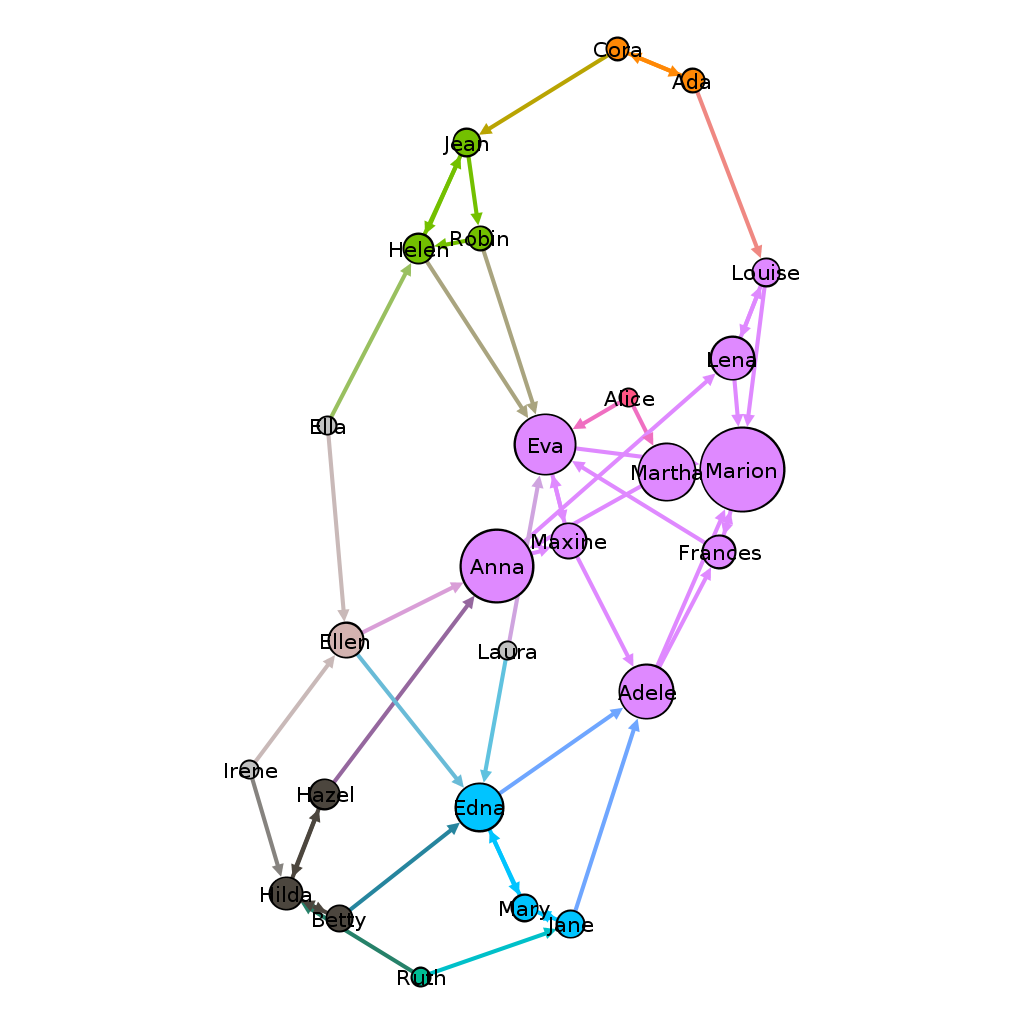
\includegraphics[width=\textwidth]{res/img/network_output}
\caption{Network representation using the highest betweenes centrality as metric}
\label{fig:network_output}
\end{figure}

\section{Facebook network}

\subsection{Question 1}

There are 388 nodes in the network and 3598 relations. The average degree is 9.273 and the person with the highest number of connections is Stanley. According to betweeness centrality calculation, the most influential person is Kelly. 

A good combination of strategies to advertise a new device could be choosing the people with the highest out-degree - the ones that can reach the highest number of persons - and highest betweeness centrality value - the ones through which most of the information flows are passing. If we had information about the exchange of messages between people, we could have an idea about the strenght of the connections (i.e. the higher number of messages, the stronger relationship). We would be able to change our marketing strategy basing ourselves on the nodes that are sending messages to the highest number of people.

\subsection{Question 2}

There are 25 communities in this network and the largest community has 90 members. If we want to spread an opinion to the largest number of people, we should choose the biggest community. However, this opinion would not affect the member of the others communities. In order to ensure the largest propagation for an opinion, we should target at least one member for each community.

\begin{figure}[!htpb]
\centering
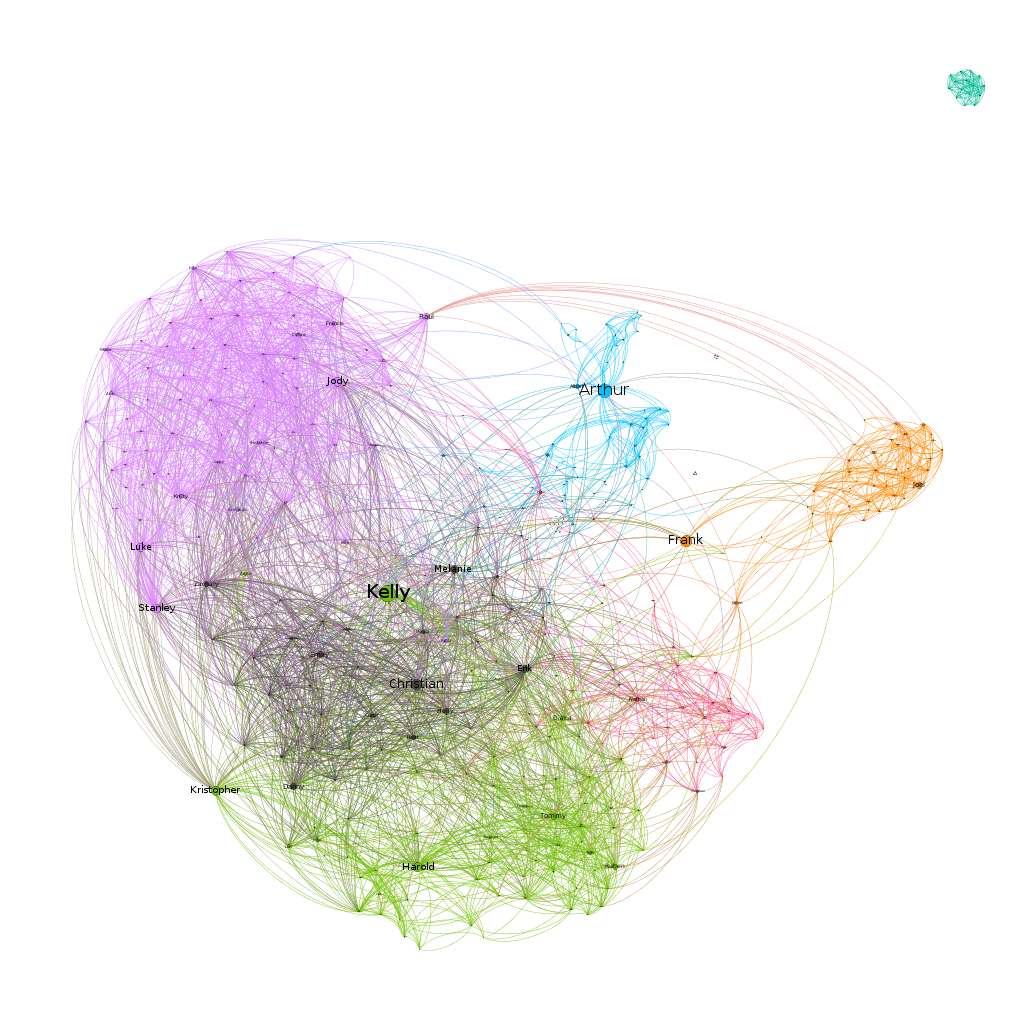
\includegraphics[width=\textwidth]{res/img/facebook}
\caption{Example of a network on Facebook highlighting communities}
\label{fig:facebook}
\end{figure}

\end{document}
